\subsection{Discovering morphological categories}
\label{sec:categories}

We know take a further step into probing the lexical knowledge of the
CNLM, asking whether this model, although it lacks explicit word
encodings, is storing information about linguistic properties of
words, such as their part of speech and number. We focus on German and
Italian, given the massive morphosyntactic ambiguities and the
impoverished morphology of English.

\paragraph{Word classes (nouns vs.~verbs)}

We sampled 500 verbs and 500 nouns from the Wikipedia training set,
requiring that they end in -\emph{en} (German) or -\emph{re}
(Italian), and that they are not tagged as both nouns and verbs in the
corpus. The first constraint sets the bar higher for methods relying
on surface cues, as all verbs and nouns share the same endings. We
randomly selected N=20 training examples, balanced between the two
classes, and tested on the remaining examples.  We repeated this
experiment 100 times to control for variation between random
train-test splits. We recorded the final hidden state of a pre-trained
CNLM after reading a word, without context, and trained a logistic
non-verb classifier on these representations.

As a baseline, we used a character-level LSTM autoencoder trained to
reconstruct individual words in isolation.  We expect that the hidden
state of the autoencoder encodes orthographic features relevant for
the languages.  We further considered word embeddings from the output
layer of the WordNLM, removing OOV words from the evaluation of this
model. Finally, we ran a version where the WordNLM was run on all words,
randomly guessing for OOV words.
%\textbf{This needs to be further discussed: can you compute  performance with random guess for OOV words?}

Results are shown in Table~\ref{tab:pos-results}.  Across the board,
models based on language models outperform the autoencoders, showing
that the former learned categories based on broader distributional
evidence, not just typical strings cuing nouns and verbs. Moreover,
the LSTM CNLM outperforms the RNN, probably because it can track
broader contexts. Not surprisingly, the word-based models fares
better, but the gap, especially in Italian, is rather narrow.

We then studied how performance evolves as we change training set size from 2 to 100. The resulting accuracy curves for German are shown in Figure~\ref{fig:pos-induction} (Italian results are qualitatively identical). They confirm that CNLM representations already distinguish the categories well for small training sets, while the autoencoder does not catch up even with 100 training examples per category.

\begin{table}[t]
  \begin{center}
    \begin{tabular}{l|l|l}
   &\emph{German}&\emph{Italian}\\
      \hline
	    LSTM & 89.0 ($\pm$ 0.14) & 95.0 ($\pm$ 0.10) \\
	    RNN & 82.0 ($\pm$ 0.64) & 91.9 ($\pm$ 0.24) \\
	    Autoencoder & 65.1 ($\pm$ 0.22) & 82.8 ($\pm$ 0.26) \\
	    WordNLM & 97.4 ($\pm$ 0.05) & 96.0 ($\pm$ 0.06) \\
	    WordNLM (all words) & 53.5 ($\pm$ 0.18)  & 62.5 ($\pm$ 0.26) \\
    \end{tabular}
  \end{center}
  \caption{\label{tab:pos-results} Word  accuracy (20 training examples per category), with standard errors computed from 100 runs.}
\end{table}


\begin{figure}
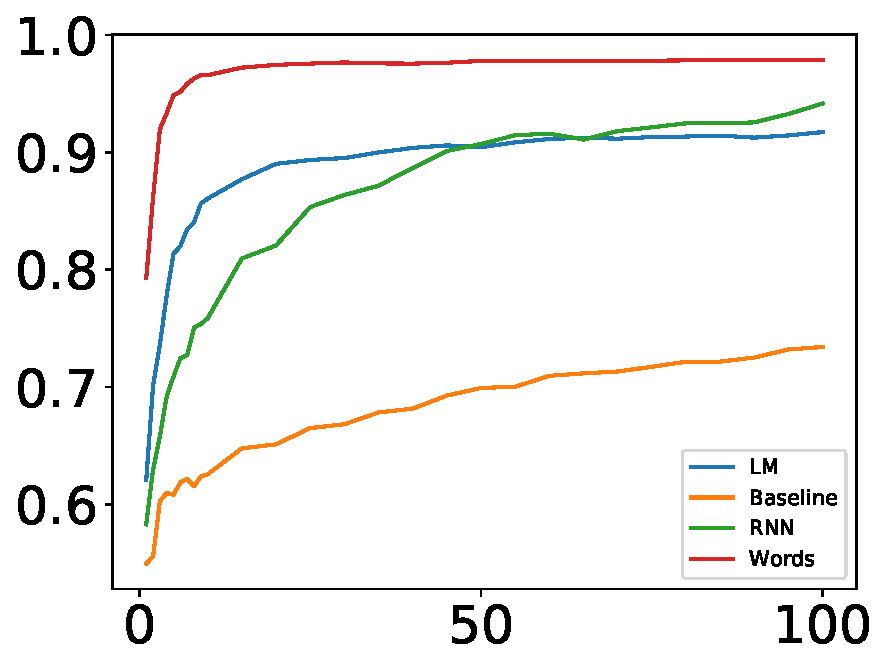
\includegraphics[width=0.48\textwidth]{figures/german_pos_nouns_verbs.pdf}
	\caption{Word class accuracy as a function of training examples (German). }\label{fig:pos-induction}
	% \textbf{Please rename LM LSTM, Baseline Autoencoder and Words WordNLM}
\end{figure}





\paragraph{Number}
We turn next to a more granular morphological feature, namely
number. We study German because of its rich system of nominal classes
that form plural through different morphological processes. We train a
number classifier on a subset of these classes, and test on the
others. If a model generalizes correctly, it means that it is
sensitive to number as an abstract feature, independently of its
surface expression.

We extracted plural nouns from the German Universal Dependencies
treebank \cite{de2006generating,mcdonald2013universal}.  We selected
nouns with plurals formed with -\emph{n}, -\emph{s}, or -\emph{e}
suffixation to train the classifier (e.g., \emph{Geschichte-n} `stories'), and tested on plurals formed with
-\emph{r} suffixation or vowel change (\emph{umlaut}, e.g. \emph{T{\"o}chter} for singular \emph{Tochter} `daughter').
%\textbf{Add one
%  example from training, one from testing.}

For the training set, we randomly selected 30 singulars and 30 plurals
from each of the training classes.  As plural suffixes make words
longer, we sampled singulars and plurals %used rejection sampling \textbf{(cite something?)}
from a
single distribution over lengths to ensure that the lengths of the
singular and plural examples were approximately matched.  For the test
set, we selected all plurals with the -\emph{r} suffix (127 items) or vowel change (38 items)
together with their respective singulars. %\textbf{(how many?)}.
To
control for the impact of random selection of training samples, we
repeat the experiment 200 times and average the resulting accuracies
on number classification.  We extract word representations as above,
and we compare to an autoencoder and embeddings from the WordNLM.
Results are summarized in Table \ref{tab:number-results}.



\begin{table}[t]
	\footnotesize
  \begin{center}
    \begin{tabular}{l|c|l|lllllll}
      &train classes&\multicolumn{2}{c}{test classes}\\
      &\emph{-n/-s/-e}&\emph{-r}&\emph{Umlaut}\\      \hline
	    LSTM& 77.9 ($\pm$ 0.8) & \textbf{88.2} ($\pm$ 0.3) & 52.8 ($\pm$ 0.6) \\
	    RNN& 70.3 ($\pm$ 0.9) & 81.3 ($\pm$ 0.7) & 53.3 ($\pm$ 0.6)\\
	    Autoencoder& 64.0 ($\pm$ 1.0) & 73.8 ($\pm$ 0.6) & 59.2 ($\pm$ 0.5)\\
	    WordNLM& \textbf{97.8 ($\pm$ 0.3)} & 86.6 ($\pm$ 0.2) & \textbf{96.7} ($\pm$ 0.2)  \\ % when including OOVs: 81.0/83.8/81.5 & 72.9 & 77.6\\
    \end{tabular}
  \end{center}
	\caption{\label{tab:number-results} German number classification accuracy, with standard errors computed from 200 runs.}
\end{table}




%\begin{table}[t]
%  \begin{center}
%    \begin{tabular}{l|l|l|lllllll}
%      &train classes&\multicolumn{2}{|c}{test classes}\\
%      &\emph{-n/-s/-e}&\emph{-r}&\emph{Umlaut}\\      \hline
%	    LSTM& 77.9 ($\pm$ 0.76) & \textbf{88.2} ($\pm$ 0.32) & 52.8 ($\pm$ 0.57) \\
%	    RNN& 70.3 ($\pm$ 0.88) & 81.3 ($\pm$ 0.72) & 53.3 ($\pm$ 0.64)\\
%	    Autoencoder& 64.0 ($\pm$ 0.96) & 73.8 ($\pm$ 0.61) & 59.2 ($\pm$ 0.47)\\
%	    WordNLM& \textbf{97.8 ($\pm$ 0.26)} & 86.6 ($\pm$ 0.15) & \textbf{96.7} ($\pm$ 0.19)  \\ % when including OOVs: 81.0/83.8/81.5 & 72.9 & 77.6\\
%    \end{tabular}
%  \end{center}
%	\caption{\label{tab:number-results} German number classification accuracy, with standard errors computed from 200 runs.}
%\end{table}
%



%\begin{table*}[t]
%  \begin{center}
%    \begin{tabular}{l|l|l|l}
%      &\multicolumn{1}{c}{train classes}&\multicolumn{2}{|c}{test classes}\\
%      &\multicolumn{1}{c}{\emph{-n/-s/-e}}&\emph{-r}&\emph{Umlaut}\\      \hline
%      LSTM& 82.1 ($\pm$ 0.74)/68.0 ($\pm$ 0.87)/83.7 ($\pm$ 0.68)  & \textbf{88.2} ($\pm$ 0.32) & 52.8 ($\pm$ 0.57) \\
%      RNN& 77.6 ($\pm$ 0.81)/60.0 ($\pm$ 0.94)/73.4 ($\pm$ 0.89) & 81.3 ($\pm$ 0.72) & 53.3 ($\pm$ 0.64)\\
%      Autoencoder& 73.2 ($\pm$ 0.97)/54.5 ($\pm$ 0.93)/64.4 ($\pm$ 0.99) & 73.8 ($\pm$ 0.61) & 59.2 ($\pm$ 0.47)\\
%	    WordNLM& \textbf{97.1 ($\pm$ 0.31)/97.9 ($\pm$ 0.27)/98.5 ($\pm$ 0.20)} & 86.6 ($\pm$ 0.15) & \textbf{96.7} ($\pm$ 0.19)  \\ % when including OOVs: 81.0/83.8/81.5 & 72.9 & 77.6\\
%    \end{tabular}
%  \end{center}
%	\caption{\label{tab:number-results} German number classification accuracy, with standard errors computed from 200 runs.}
%\end{table*}

%python char-lm-ud-stationary-separate-bidir-with-spaces-probe-baseline-prediction-wiki-plurals-2-tests-RNN.py  --batchSize 256 --char_dropout_prob 0.01 --char_embedding_size 50 --char_noise_prob 0.0 --hidden_dim 2048 --language german --layer_num 2 --learning_rate 0.1 --nonlinearity tanh --load-from wiki-german-nospaces-bptt-rnn-237671415 --sequence_length 30 --weight_dropout_hidden 0.0 --weight_dropout_in 0.0
%python char-lm-ud-stationary-separate-bidir-with-spaces-probe-baseline-prediction-wiki-plurals-2-tests-words.py  --language german --batchSize 128 --char_embedding_size 200 --hidden_dim 1024 --layer_num 2 --weight_dropout_in 0.1 --weight_dropout_hidden 0.35 --char_dropout_prob 0.0 --char_noise_prob 0.01 --learning_rate 0.2 --load-from wiki-german-nospaces-bptt-words-966024846


The classifier based on word embeddings is overall the most
successful, confirming that word embeddings encode number reliably
\cite{Mikolov:etal:2013a}.  CNLM encodings outperform the autoencoder
on plurals formed with suffixes, indicating some capability to
generalize to unseen plurals that go beyond relying on orthographic
cues.  For -\emph{r} plurals, the CNLM LSTM even generalizes better
than the WordNLM.  In contrast, almost no generalization to plurals
formed by vowel change is found (the CNLMs are \emph{worse} than the
autoencoder here), suggesting that the CNLM number encoding is not
general enough to generalize across very different surface
morphological processes (adding a suffix vs.~changing the root vowel).
